\scanpage{51}
% archive sheet number: 50
\unsure{Sous-algèbre|Sous-algèbres} \unsure{tautologique|tautologiques} \unsure{des|de} $H^*(X^n)$.

\textcircled{1} \uline{$H^*(X)$}\qquad\deleted{degrés}

\diagram{$\begin{array}{lll}
 \text{\uline{générateurs}} & y\in H^{\unsure{n|m}}(X) &\\
 \text{\uline{relation}s} & y^2=0 &\\
 \text{\uline{base}} & \text{deg. }0 &1\\
 &\text{deg. }n &y
\end{array}$}

\textcircled{2} \uline{$H^*(X\times X)$}

\uline{générateurs}:\qquad $y\otimes1=y_1$ \deleted{\unsure{1}}, $1\otimes y=y_2$, $\delta\qquad\in H^n(X)$

\uline{relations}\qquad $y_1^2=y_2^2=0$, $y_1y_2=y_1\delta=y_2\delta$; $\delta^2=\chi\,y_1y_2$\qquad
($\chi\in\mathbb{Z}$ la \unsure{car|car.} d'EP)

\diagram{$\begin{array}{lll}
 \text{\uline{base}} & \text{deg }0 &1\\
 &\text{deg }n &y_1,y_2,\delta\\
 &\text{deg }2n &y_1y_2y_3
\end{array}$}

\textcircled{3} $H^*(X\times X\times X)$

\diagram{$\begin{array}{lll}
 \text{\uline{générateurs}} & \text{degr }n:\ \cdot &
 y\otimes1\otimes1=y_1,\quad 1\otimes y\otimes1=y_2,\quad 1\otimes1\otimes y=y_3,\quad
 \delta_{12}=\delta\otimes1,\delta_{23},\delta_{31}\\
 &\text{deg }2n &\delta
\end{array}$}

\uline{relations}
\[
\left\{\begin{aligned}
 &y_1^2=y_2^2=y_3^2=0\\
 &\delta_{12}^2=\chi\,y_1y_2,\ \delta_{23}^2=\chi\,y_2y_3,\ \delta_{31}^2=\chi\,y_3y_1,\ 
 \delta_{12}\delta_{23}=\delta_{12}\delta_{31}=\delta_{23}\delta_{31}=\delta\\
 &\delta_{12}y_1=\delta_{12}y_2=\deleted{\unsure{\delta}}y_1y_2,\ 
 \delta_{23}y_2=\delta_{23}y_3=y_2y_3,\ \delta_{31}y_3=\delta_{31}y_1=y_3y_1\\
 &\delta y_1=\delta y_2=\delta y_3=y_1y_2y_3\\
 &\delta^2=0\\
 &\delta_{12}\delta=\delta_{23}\delta=\delta_{31}\delta=\chi\,y_1y_2y_3
\end{aligned}\right.
\]
\diagram{$\begin{array}{lll}
 \text{\uline{base}} &\text{deg }0&1\\
 &\text{deg }n&y_1,y_2,y_3,\delta_{12},\delta_{23},\delta_{31}\\
 &\text{deg }2n&y_1y_2,y_2y_3,y_3y_1,\delta_{12}y_3,\delta_{23}y_1,\delta_{31}y_2,\delta\\
 &\text{deg }3n&y_1y_2y_3
\end{array}$}

\figure{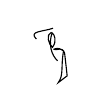
\begin{tikzpicture}[x=0.23cm,y=0.23cm]
 \draw[thin] (0,2.7) .. controls (-.45,3.15) and (.35,3.1) .. (.92,3.3);
 \draw (.83,3.08) .. controls (.51,2.95) and (.67,2.40) .. (.89,2.25)
 .. controls (1.16,2.6) and (.98,2.99) .. (.87,3.04)
 .. controls (.65,2.43) and (.83,1.81) .. (1.17,1.50);
 \draw (.94,2.14) .. controls (1.23,2.25) and (1.38,2.14) .. (1.5,2.05)
 .. controls (1.34,1.15) and (1.52,.72) .. (1.21,.30)
 -- (1.70,.67) -- (1.56,1.92)
 .. controls (1.43,2.35) and (1.1,2.02) .. (.94,2.14);
\end{tikzpicture}}

